
\chapter{Math}
\label{cha:probability}

\section{Markov chain}
\label{sec:markov-chain}

A \keyword{Markov chain} or \keyword{Markov process} is a stochastic model describing a sequence of possible events in which the probability of each event depends only on the state attained in the previous event.

\subsection{Transitions}
\label{sec:transitions}

The changes of state of the system are called \keyword{transitions}.
The probabilities associated with various state changes are called \keyword{transition probabilities}.
The process is characterized by a state space, a transition matrix describing the probabilities of particular transitions, and an initial state (or initial distribution) across the state space.

\subsection{Discrete-time Markov chain}
\label{sec:discrete-time-markov}

A \keyword{discrete-time Markov chain} is a sequence of random variables $X_1, X_2, X_3, \ldots$ with the Markov property, namely that the probability of moving to the next state depends only on the present state and not on the previous states:
\begin{equation}
  \label{eq:14}
   \operatorname{P}\left(X_{n+1}=x \mid X_1=x_1, X_2=x_2, \ldots, X_n=x_n\right)=\operatorname{P}\left(X_{n+1}=x \mid X_n=x_n\right)
\end{equation}

if both conditional probabilities are well defined, that is, if \(\operatorname{P}\left(X_1=x_1, \ldots, X_n=x_n\right)>0\).



The possible values of $X_i$ form a countable set $S$ called the state space of the chain.


\subsection{Continous-time Markov chain}
\label{sec:cont-time-mark}

A \keyword{continuous-time Markov chain} $\mathrm{X}(\mathrm{t})$ is defined by two components: a jump chain, and a set of holding time parameters $\lambda_i$.
The jump chain consists of a countable set of states $\mathrm{S} \subset\{0,1,2, \cdots\}$ along with transition probabilities $\mathrm{p}_{\mathrm{ij}}$.
We assume $\mathrm{p}_{\mathrm{ii}}=0$, for all non-absorbing states $\mathrm{i} \in \mathrm{S}$.
We assume
\begin{enumerate}
\item if $X(t)=i$, the time until the state changes has Exponential $\left(\lambda_{\mathrm{i}}\right)$ distribution;
\item if $X(t)=i$, the next state will be $j$ with probability $p_{i j}$.
\end{enumerate}

The process satisfies the Markov property.
That is, for all $0 \leq \mathrm{t}_1<\mathrm{t}_2<\cdots<\mathrm{t}_{\mathrm{n}}<\mathrm{t}_{\mathrm{n}+1}$, we have
$$
\begin{aligned}
\mathrm{P}\left(\mathrm{X}\left(\mathrm{t}_{\mathrm{n}+1}\right)=\mathrm{j} \mid \mathrm{X}\left(\mathrm{t}_{\mathrm{n}}\right)\right. & \left.=\mathrm{i}, \mathbf{X}\left(\mathrm{t}_{\mathrm{n}-1}\right)=\mathrm{i}_{\mathrm{n}-1}, \cdots, X\left(\mathrm{t}_1\right)=\mathrm{i}_1\right) \\
& =\mathrm{P}\left(\mathrm{X}\left(\mathrm{t}_{\mathrm{n}+1}\right)=\mathrm{j} \mid \mathbf{X}\left(\mathrm{t}_{\mathrm{n}}\right)=\mathrm{i}\right)
\end{aligned}
$$


\subsection{Markov kernel}
\label{sec:markov-kernel}


Let $(X, \mathcal{A})$ and $(Y, \mathcal{B})$ be \keyword{measurable spaces}.
A \keyword{Markov kernel} with source $(X, \mathcal{A})$ and target $(Y, \mathcal{B})$ is a map $\kappa: \mathcal{B} \times X \rightarrow[0,1]$ with the following properties:
\begin{enumerate}
\item For every (fixed) $B \in \mathcal{B}$, the map $x \mapsto \kappa(B, x)$ is $\mathcal{A}$-measurable
\item For every (fixed) $x \in X$, the map $B \mapsto \kappa(B, x)$ is a \keyword{probability measure} on $(Y, \mathcal{B})$
\end{enumerate}

In other words it associates to each point $x \in X$ a probability measure $\kappa(d y \mid x): B \mapsto \kappa(B, x)$ on $(Y, \mathcal{B})$ such that, for every measurable set $B \in \mathcal{B}$, the map $x \mapsto \kappa(B, x)$ is measurable with respect to the $\sigma$-algebra $\mathcal{A}$.


\subsection{Measurable space}
\label{sec:measurable-space}

A \keyword{measurable space} consists of a set and a \keyword{\(\sigma\)-algebra}, which defines the subsets that will be measured.

Consider a set \(X\) and a \(\sigma\)-algebra \(\mathcal{A}\) on \(X\).
Then the tuple \((X, \mathcal{A})\) is called a measurable space.

\subsection{\protect{\(\sigma\)}-algebra}


A \keyword{\(\sigma\)-algebra} (also \(\sigma\)-field) on a set \(X\) is a nonempty collection \(\Sigma\) of subsets of \(X\) closed under complement, countable unions, and countable intersections.

Let $X$ be some set, and let $P(X)$ represent its power set.
Then a subset $\Sigma \subseteq P(X)$ is called a $\sigma$-algebra if it satisfies the following three properties:
\begin{enumerate}
\item $X$ is in $\Sigma$, and $X$ is considered to be the universal set in the following context.
\item $\Sigma$ is closed under complementation: If $A$ is in $\Sigma$, then so is its complement, $X \backslash A$.
\item $\Sigma$ is closed under countable unions: If $A_1, A_2, A_3, \ldots$ are in $\Sigma$, then so is $A=A_1 \cup A_2 \cup A_3 \cup \cdots$.
\end{enumerate}

From these properties, it follows that the $\sigma$-algebra is also closed under countable intersections (by applying De Morgan's laws).

\section{Conditional probability}
\label{sec:cond-prob}

Given two events \(A\) and \(B\).

\begin{equation}
  \label{eq:19}
  P(A \mid B)=\frac{P(A \cap B)}{P(B)}
\end{equation}

\(P(A|B)\) stands for the probability of A happening given that B happened.
\(P(A \cap B)\) stands for the probability of A and B happening at the same time.
\(P(B)\) stands for the probability of B happening.
\section{Posterior probability}
\label{sec:post-prob}

The \keyword{posterior probability} is a type of conditional probability that results from updating the prior probability with information summarized by the likelihood via an application of Bayes' rule.

In variational Bayesian methods, the posterior probability is the probability of the parameters $\theta$ given the evidence $X$, and is denoted $p(\theta \mid X)$.
It contrasts with the likelihood function, which is the probability of the evidence given the parameters: $p(X \mid \theta)$.

The two are related as follows:
Given a prior belief that a probability distribution function is $p(\theta)$ and that the observations $x$ have a likelihood $p(x \mid \theta)$, then the posterior probability is defined as

\begin{equation}
  \label{eq:20}
  p(\theta \mid x)=\frac{p(x \mid \theta)}{p(x)} p(\theta)  
\end{equation}

where $p(x)$ is the normalizing constant and is calculated as
\begin{equation}
  \label{eq:21}
  p(x)=\int p(x \mid \theta) p(\theta) d \theta  
\end{equation}




\section{Guassian distribution}
\label{sec:guass-distr}


\keyword{Gaussian distribution} (normal distribution) is a type of continuous probability distribution for a real-valued random variable.
The general form of its probability density function is
\begin{equation}
  \label{eq:22}
  f(x)=\frac{1}{\sigma \sqrt{2 \pi}} e^{-\frac{1}{2}\left(\frac{x-\mu}{\sigma}\right)^2}  
\end{equation}


The parameter $\mu$ is the mean or expectation of the distribution (and also its median and mode), while the parameter $\sigma$ is its standard deviation.
The variance of the distribution is $\sigma^2$.
The Figure \ref{fig:gaussian-distribution} shows the Gaussian distributions.

\begin{figure}[!htp]
  \centering
  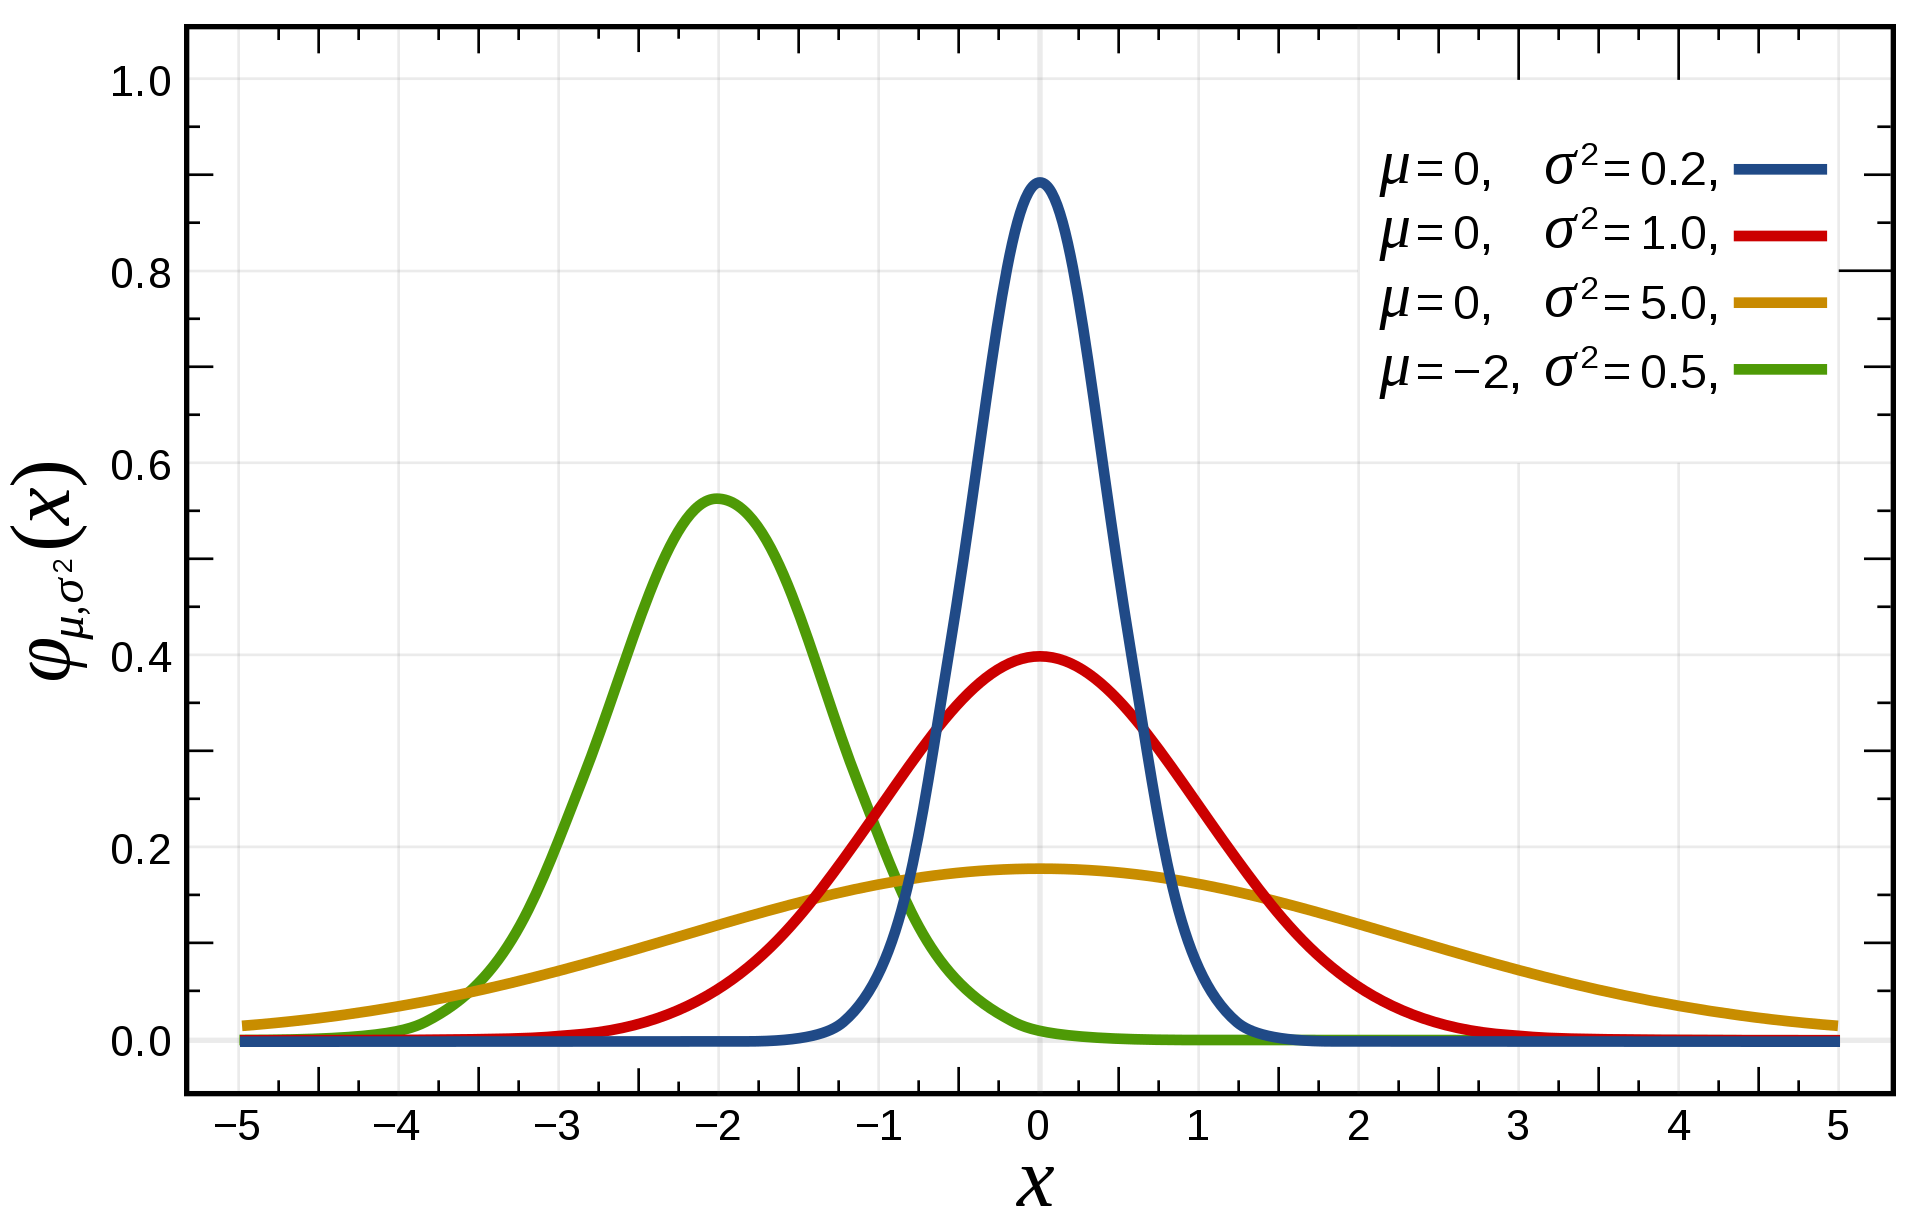
\includegraphics[width=0.8\textwidth]{images/gaussian-distribution}
  \caption{Gaussian distribution}
  \label{fig:gaussian-distribution}
\end{figure}
\section{Laplace distribution}
\label{sec:laplace-distribution}

A random variable has a Laplace $(\mu, b)$ distribution if its probability density function is
\begin{equation}
  \label{eq:23}
  f(x)=\frac{1}{2 b} \exp \left(-\frac{|x-\mu|}{b}\right)  
\end{equation}

Here \(\mu\) is a location parameter and \(b\) is a scale parameter.
Figure \ref{fig:laplace-distribution} shows the Laplace distributions.

\begin{figure}[!htp]
  \centering
  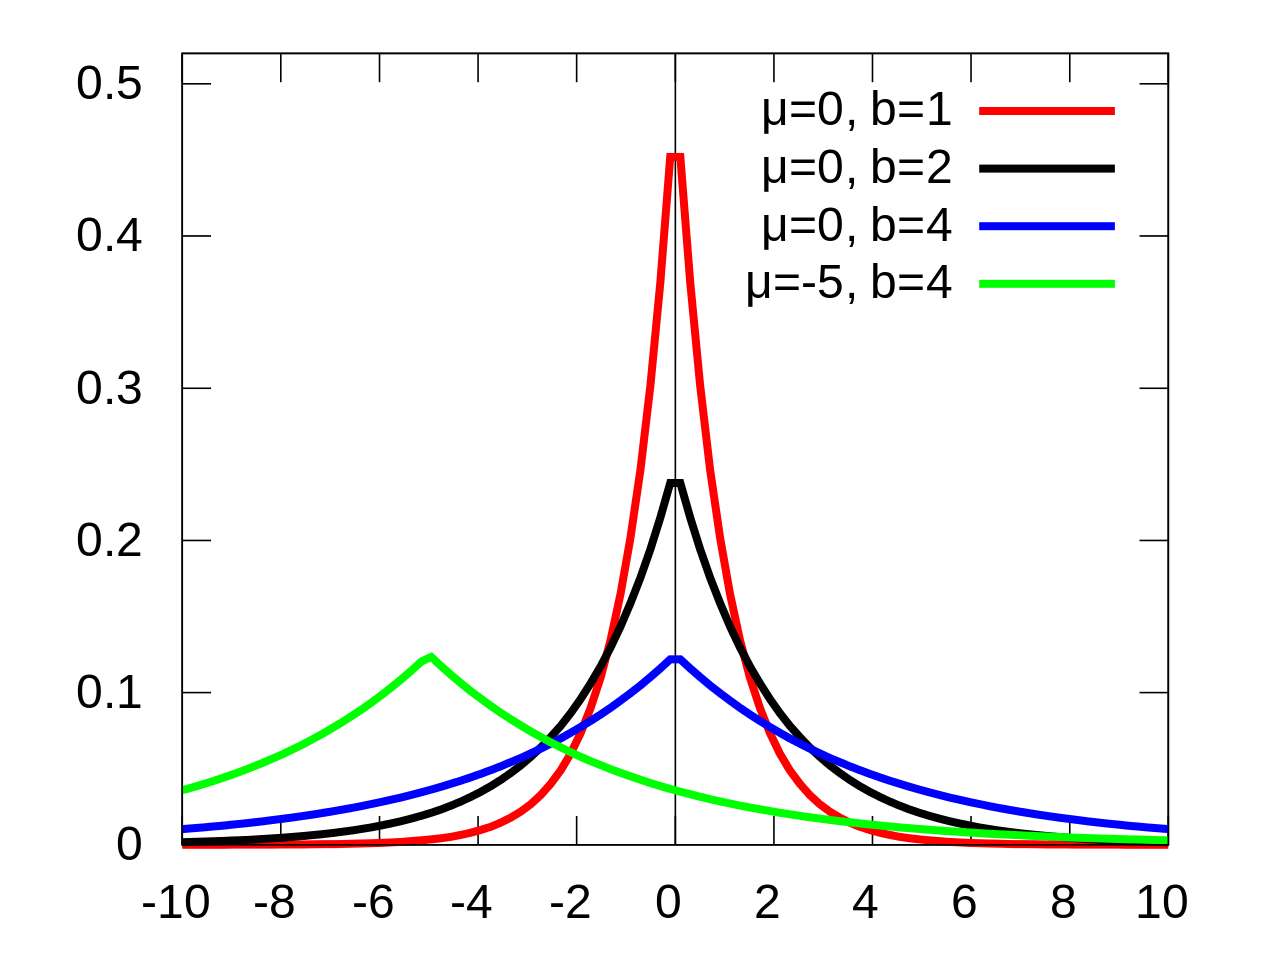
\includegraphics[width=0.8\textwidth]{images/laplace-distribution}
  \caption{Laplace distribution}
  \label{fig:laplace-distribution}
\end{figure}

\section{Monte Carlo method}
\label{sec:monte-carlo-method}

\keyword{Monte Carlo methods} are a broad class of computational algorithms that rely on repeated random sampling to obtain numerical results.
The underlying concept is to use randomness to solve problems that might be deterministic in principle.


Monte Carlo methods vary, but tend to follow a particular pattern:
\begin{enumerate}
\item Define a domain of possible inputs
\item Generate inputs randomly from a probability distribution over the domain
\item Perform a deterministic computation on the inputs
\item Aggregate the results
\end{enumerate}



\section{Variational Bayesian methods}
\label{sec:vari-bayes-meth}


It is a simplifying that makes the intractable events into tractable events.

For example,
in variational inference, the posterior distribution over a set of unobserved variables $\mathbf{Z}=\left\{Z_1 \ldots Z_n\right\}$ given some data $\mathbf{X}$ is approximated by a so-called variational distribution, $Q(\mathbf{Z})$:
\begin{equation}
  \label{eq:26}
  P(\mathbf{Z} \mid \mathbf{X}) \approx Q(\mathbf{Z})  
\end{equation}


The distribution $Q(\mathbf{Z})$ is restricted to belong to a family of distributions of simpler form than $P(\mathbf{Z} \mid \mathbf{X})$ (e.g. a family of Gaussian distributions), selected with the intention of making $Q(\mathbf{Z})$ similar to the true posterior, $P(\mathbf{Z} \mid \mathbf{X})$.

The similarity (or dissimilarity) is measured in terms of a dissimilarity function $d(Q ; P)$ and hence inference is performed by selecting the distribution $Q(\mathbf{Z})$ that minimizes $d(Q ; P)$.
The most common type of variational Bayes uses the Kullback-Leibler divergence (KL-divergence) of $Q$ from $P$ as the choice of dissimilarity function. 

\section{Bayesian probability}
\label{sec:bayesian-probability}

Bayesian probability is an interpretation of the concept of probability, in which, instead of frequency or propensity of some phenomenon, probability is interpreted as reasonable expectation representing a state of knowledge or as quantification of a personal belief.

\section{Binomial distribution}
\label{sec:binom-distr}

In general, if the random variable $X$ follows the binomial distribution with parameters $n \in \mathbb{N}$ and $p \in$ $[0,1]$, we write $X \sim \mathrm{B}(n, p)$.
The probability of getting exactly $k$ successes in $n$ independent Bernoulli trials is given by the probability mass function:
\begin{equation}
  \label{eq:24}
  f(k)=\left(\begin{array}{l}
               n \\
               k
             \end{array}\right) p^k(1-p)^{n-k}
\end{equation}

for $k=0,1,2, \ldots, n$, where
\begin{equation}
  \label{eq:25}
\left(\begin{array}{l}
n \\
k
\end{array}\right)=\frac{n !}{k !(n-k) !}
\end{equation}

The figure \ref{fig:binomial-distribution} shows the distribution.
\begin{figure}[!htp]
  \centering
  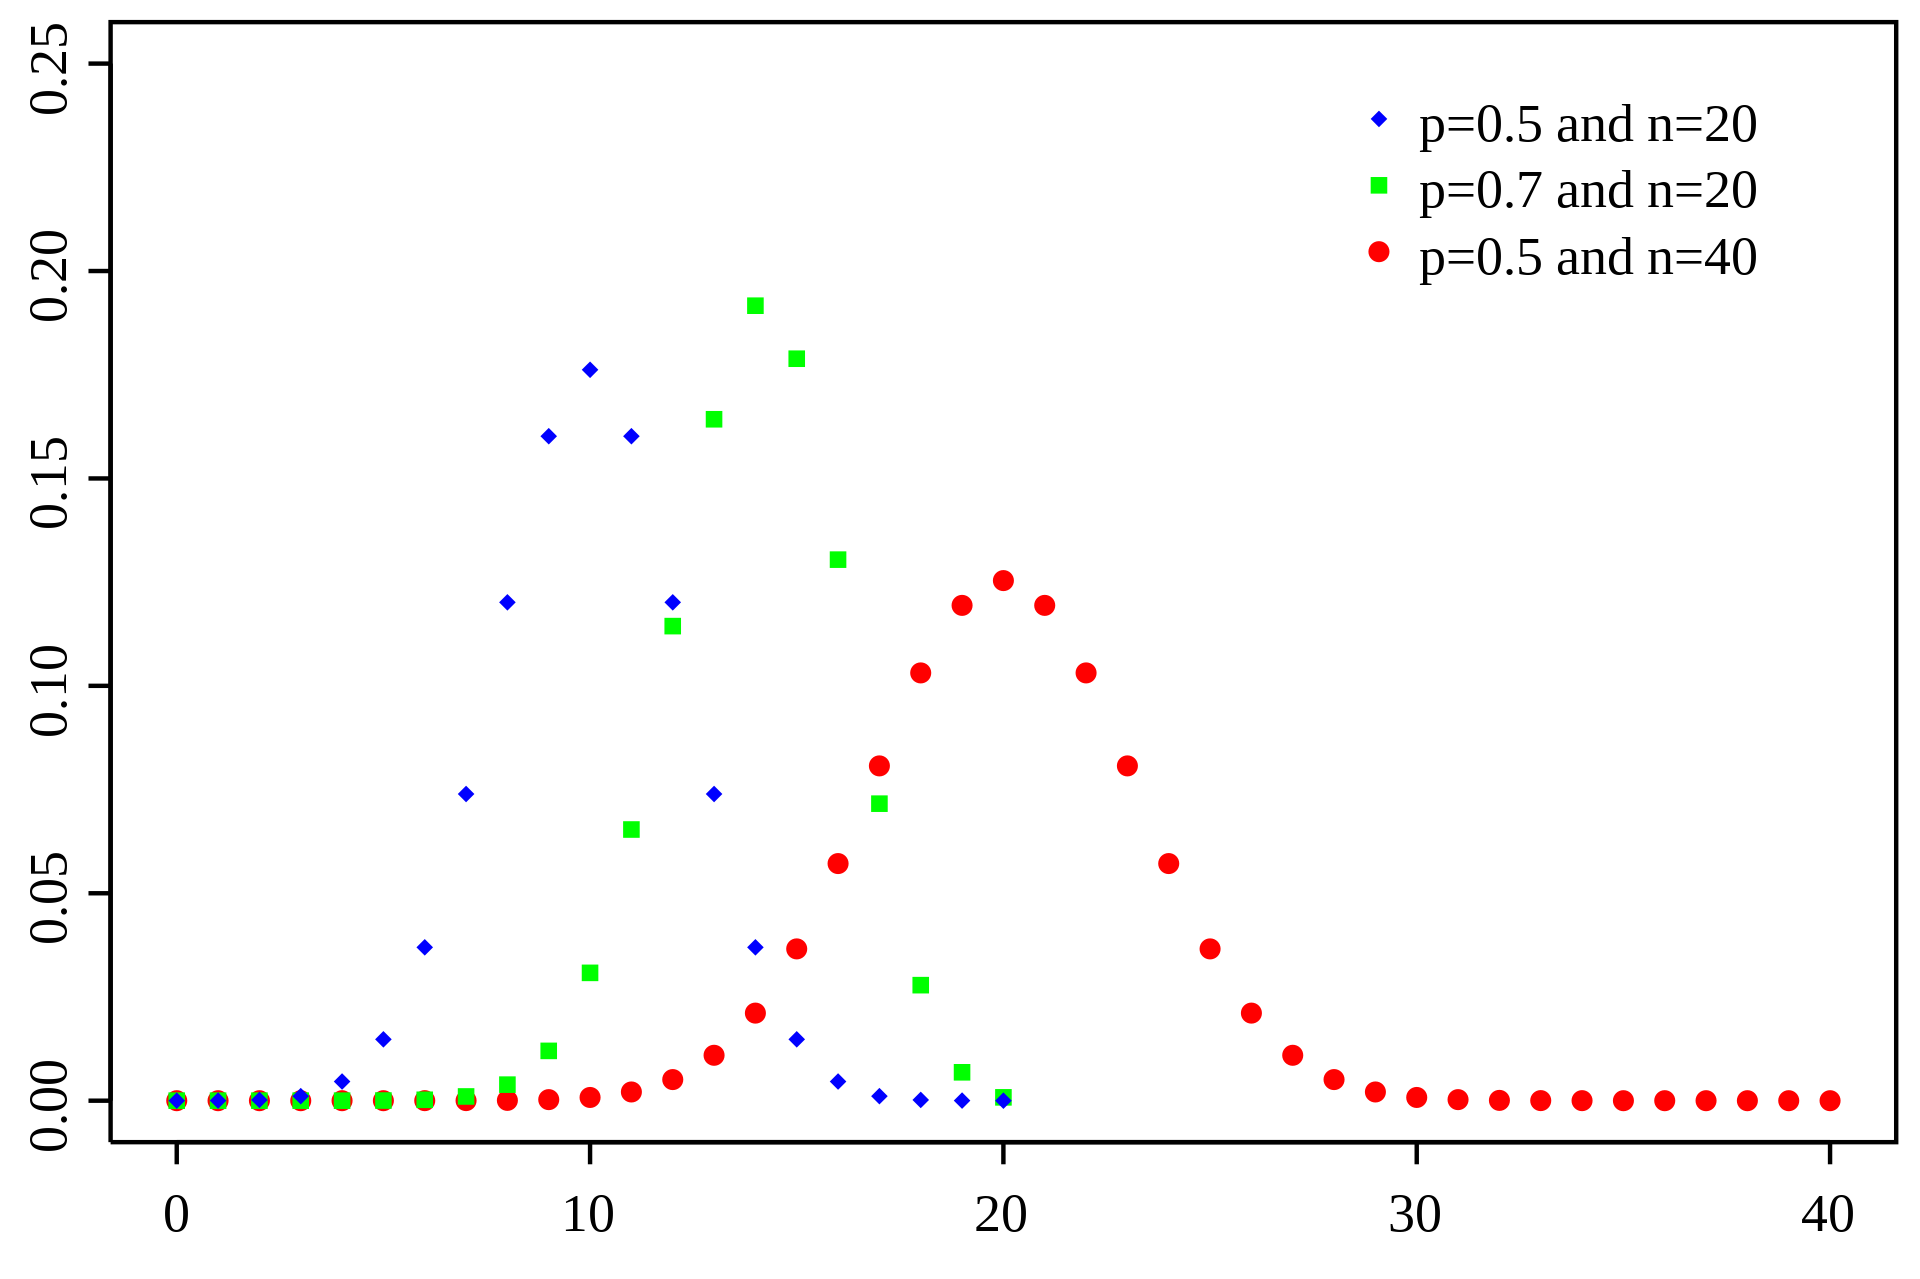
\includegraphics[width=0.6\textwidth]{images/binomian-distribution.png}
  \caption{Binomial distribution}
  \label{fig:binomial-distribution}
\end{figure}

\section{Kullback–Leibler divergence}
\label{sec:kullb-diverg}


The Kullback-Leibler divergence, denoted $D_{\mathrm{KL}}(P \| Q)$, is a type of statistical distance: a measure of how one probability distribution $P$ is different from a second, reference probability distribution $Q$.


For discrete probability distributions $P$ and $Q$ defined on the same sample space, $\mathcal{X}$, the relative entropy from $Q$ to $P$ is defined ${ }^{[11]}$ to be
\begin{equation}
  \label{eq:27}
  D_{\mathrm{KL}}(P \| Q)=\sum_{x \in \mathcal{X}} P(x) \log \left(\frac{P(x)}{Q(x)}\right) .  
\end{equation}


which is equivalent to
\begin{equation}
  \label{eq:28}
  D_{\mathrm{KL}}(P \| Q)=-\sum_{x \in \mathcal{X}} P(x) \log \left(\frac{Q(x)}{P(x)}\right)  
\end{equation}

\section{Jensen's inequality}
\label{sec:jensens-inequality}

Jensen's inequality generalizes the statement that a secant line of a convex function lies above its graph.

Thus, Jensen's inequality is
\begin{equation}
  \label{eq:40}
f\left(t x_1+(1-t) x_2\right) \leq t f\left(x_1\right)+(1-t) f\left(x_2\right) .  
\end{equation}

Shown in Figure \ref{fig:jenson-equality}.

\begin{figure}[!htp]
  \centering
  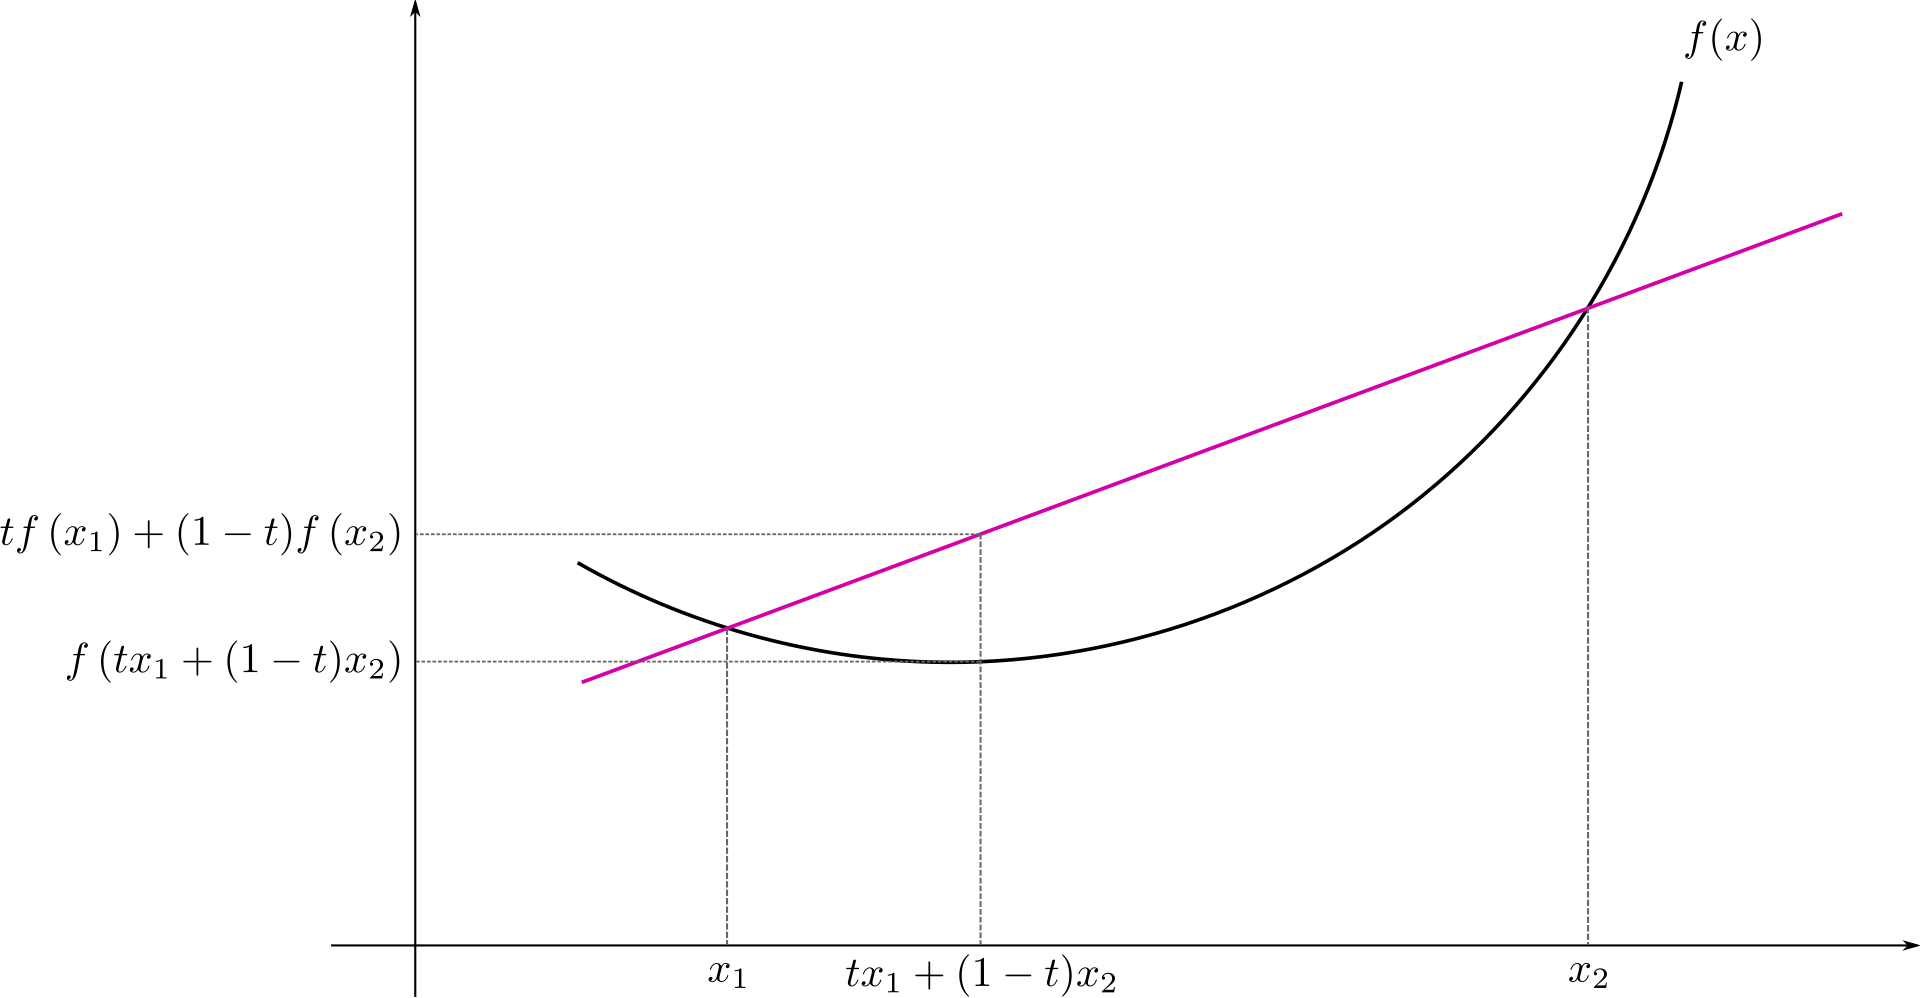
\includegraphics[width=0.6\textwidth]{images/jensen-inequality.png}
  \caption{Jensen's inequality}
  \label{fig:jenson-equality}
\end{figure}


In the context of probability theory, it is generally stated in the following form: if $X$ is a random variable and $\varphi$ is a convex function, then
\begin{equation}
  \label{eq:41}
\varphi(\mathrm{E}[X]) \leq \mathrm{E}[\varphi(X)]  
\end{equation}

The difference between the two sides of the inequality, $\mathrm{E}[\varphi(X)]-\varphi(\mathrm{E}[X])$, is called the Jensen gap.



%%% Local Variables:
%%% mode: latex
%%% TeX-master: "machine-learning"
%%% End:
